
\begin{figure}[tb]
  \centering
  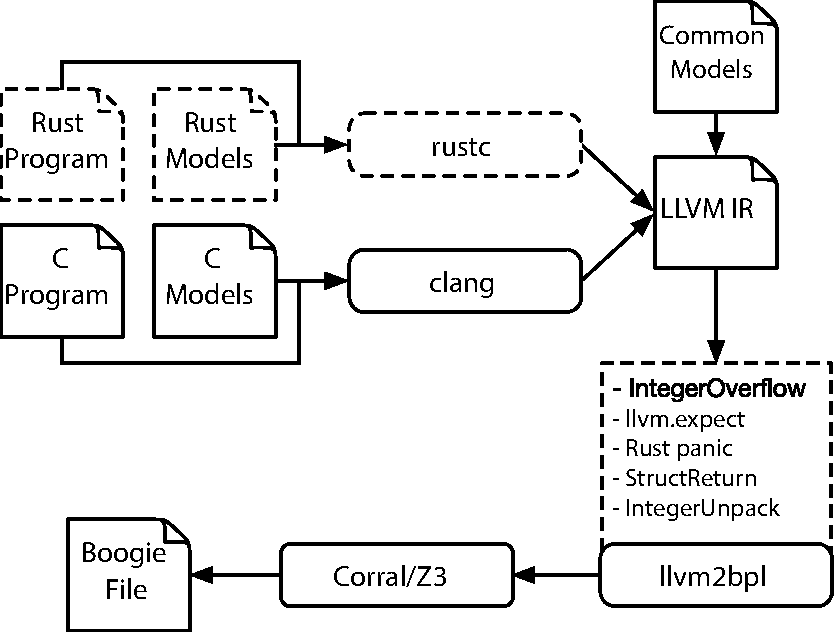
\includegraphics[width=0.99\textwidth]{RustSmack}
  \caption{Toolflow of SMACK.}
  \label{fig:atvatoolflow}
\end{figure}

SMACK~\cite{smack14,smack} is a software verification toolchain that translates
LLVM IR code into Boogie intermediate verification language~\cite{boogie},
which is in turn verified using back-end Boogie verifiers such as
Corral~\cite{corral}.
%
Before our Rust effort, SMACK had been predominantly used to verify LLVM IR
programs produced by the Clang C compiler.
%
\Cref{fig:atvatoolflow} shows the toolflow of SMACK, which works as follows:
%
\begin{enumerate}
\item The SMACK top-level script automates the entire toolflow. It
  determines which compiler to invoke and flags to use for
  program compilation. In the case of C programs, it invokes Clang
  to generate LLVM IR code, while including SMACK's C language models.
  The models specify the semantics of common C library functions
  such as malloc, free, and string operations.
\item The common models file is then linked with the generated LLVM IR file to
  provide basic verification capabilities. This includes
  modeling dynamic memory allocation, supporting assertions and
  assumptions, and generating nondeterministic values.
\item The core \textsc{llvm2bpl} component takes an LLVM IR file as input, and
  produces Boogie code that captures the semantics of LLVM IR instructions;
  it outputs a Boogie file for verification.
\item Finally, the Corral back-end verifier is invoked on the generated Boogie
  file, and it uses Z3~\cite{z3} as its SMT solver. (Note that SMACK supports
  other back-end verifiers, which we omitted here.)
\end{enumerate}
%
In this work, we use Corral in its bounded verification mode, meaning that it
unrolls loops and recursion up to a certain user-provided bound.

